\documentclass[12pt,a4paper]{article}
\usepackage{fullpage}
\usepackage[top=2cm, bottom=4.5cm, left=2.5cm, right=2.5cm]{geometry}
\usepackage{amsmath,amsthm,amsfonts,amssymb,amscd}
\usepackage{lastpage}
\usepackage{enumerate}
\usepackage{fancyhdr}
\usepackage{mathrsfs}
\usepackage{xcolor}
\usepackage{graphicx}
\usepackage{listings}
\usepackage{hyperref}
\usepackage{txfonts}
\usepackage{titlesec}
\usepackage{esint}

\hypersetup{%
  colorlinks=true,
  linkcolor=blue,
  linkbordercolor={0 0 1}
}


\newcommand\course{8.03x - Vibrations and Waves}
\newcommand\hwnumber{1}               
\newcommand\MyName{Syed Suhaib Ahmad}
 
\renewcommand\lstlistingname{Algorithm}
\renewcommand\lstlistlistingname{Algorithms}
\def\lstlistingautorefname{Alg.}

\setlength{\parindent}{0.0in}
\setlength{\parskip}{0.05in}



\pagestyle{fancyplain}
\headheight 35pt
\lhead{\course}
\chead{\large\textbf{Problem Set 6}}
\rhead{\MyName{}}
\lfoot{}
\cfoot{\small\thepage}
\rfoot{}
\headsep 1.5em

\begin{document}

\subsubsection*{Problem 6.1 - Phase and group velocity in your bathtub}
\begin{enumerate}
    \item[(a)]Prove that for wavelength much less than 1.7\,cm, the group velocity is 1.5 times the phase velocity (use eq. 33).
    \item[(b)]Prove that for wavelengths much greater than 1.7\,cm, the group velocity is half the phase velocity.
\end{enumerate}
\textbf{Solution(a)}
\\
\\The dispersion relation for surface waves on a deep liquid is given by the expression
\begin{equation}
    \omega^2=gk+\frac{T}{\rho}k^3,
\end{equation}
where $g$ is acceleration due to gravity, $T$ is the surface tension, and $\rho$ is density of the liquid. For $\lambda\ll1.7\,$cm, the second term ($Tk^3/\rho$) dominates and thus we can approximate the phase velocity for this scenario to be
\[v_p=\frac{\omega}{k}\approx\frac{\sqrt{Tk^3/\rho}}{k}=\sqrt{\frac{T}{\rho}k}.\]
The group velocity is given by the derivative of $\omega$ with respect to $k$.
\[v_g=\frac{d\omega}{d k}\approx\frac{d}{d k}\left(\sqrt{\frac{T}{\rho}k^3}\right)=\frac{3}{2}\sqrt{\frac{T}{\rho}k}=\frac{3}{2}v_p.\]
\textbf{Solution(b)}
\\
\\Similarly, for $\lambda\gg1.7\,$cm, the first term dominates and Eq. (1) can be approximated to $\omega^2\approx gk$. The phase velocity for this case is
\[v_p=\frac{\omega}{k}\approx\frac{\sqrt{gk}}{k}=\sqrt{\frac{g}{k}}\]
and the group velocity is
\[v_g=\frac{d\omega}{d k}\approx\frac{d}{d k}\left(\sqrt{gk}\right)=\frac{1}{2}\sqrt{\frac{g}{k}}=\frac{1}{2}v_p.\]

\subsubsection*{Problem 6.2 - Why are deep-water waves dispersive?}
Consider a U-tube of uniform cross section with two vertical arms. Let the total length of the liquid column be $l$. Imagine the liquid to be oscillating back and forth, so that at any instant the levels in the side are at $\pm y$ with respect to the equilibrium level, and all the liquid has the speed $dy/dt$.
\begin{figure}[h]
    \centering
    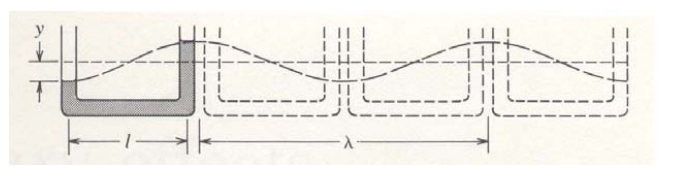
\includegraphics[width=0.75\linewidth]{figs/fig_prob_6.2.png}
    %\caption{Caption}
   % \label{fig:enter-label}
\end{figure}
\begin{enumerate}
    \item[(a)]Write down an expression for the potential energy plus kinetic energy of the liquid, and hence show that the period of oscillation is $\pi\sqrt{2l/g}$.
    \item[(b)]Imagine that a succession of such tubes can be used to define a succession of crests and troughs as in a water wave (see the diagram). Taking the result of (a), and the condition $\lambda\approx2l$ implied by this analogy, deduce that the speed of waves on water is something like $(g\lambda)^{1/2}/\pi$. (Assume that only a small fraction of the liquid is in the vertical arms of the U-tube.)
    \item[(c)]Use the exact result, $v=(g\lambda/2\pi)^{1/2}$, to calculate the speed of waves of wavelength 500\,m in the ocean.
\end{enumerate}
\textbf{Solution(a)}
\\
\\Assuming there is no damping due to resistive forces, the energy of the total energy of the system remains constant and can be determined by adding the potential and kinetic energies.
\[E=U+K=mgh+\frac{1}{2}mv^2=\rho Agy^2+\frac{1}{2}\rho Al\left(\frac{dy}{dt}\right)^2.\]
As mentioned above, the total energy remains constant.
\[\frac{\partial E}{\partial t}=0\Rightarrow\rho A\frac{dy}{dt}\left(2gy+l\frac{d^2y}{dt^2}\right)=0\]
\begin{equation}
    \Rightarrow\frac{d^2y}{dt^2}+\frac{2g}{l}y=0.
\end{equation}
Eq. (2) shows a simple harmonic oscillation with a period of $\pi\sqrt{2l/g}$ as required.
\\
\\\textbf{Solution(b)}
\\
\\The frequency of such water waves (using the result from part a) is $f=\sqrt{g/2l}/\pi$ and the speed is given by
\[v=f\lambda\approx\frac{\sqrt{g/2l}}{\pi}\times2l\approx\frac{\sqrt{g\lambda}}{\pi}.\]
\textbf{Solution(c)}
\\
\\Substituting the values into the given result gives $v\approx28$\,ms$^{-1}$.
\subsubsection*{Problem 6.3 - Energy in waves}
The energy $E_\lambda$ stored in one wavelength ($\lambda$) of a vibrating string (standing wave) is:
\[E_\lambda=\frac{TA^2\pi^2}{\lambda}\]
where $T$ is the tension in the string and $A$ is the amplitude of the anti-nodes.
\begin{enumerate}
    \item[(a)]Prove that this result is equivalent to eq. 7-38 in French (page 242). 
\end{enumerate}
If we, for simplicity, approximate a sine-wave by triangles (see figures) then we can easily calculate how much energy it takes to give the string this triangular shape.
\\You pick up the string of length $L$ in the middle $M$ (see figure above) and move this point a distance $A$ up. Assume that in doing so the tension $T$ in the string does not change ($A\ll L$).
\begin{enumerate}
    \item[(b)]Calculate the amount of work that you have to do.
\end{enumerate}
\begin{figure}[h]
    \centering
    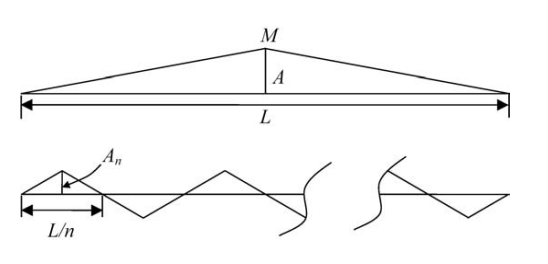
\includegraphics[width=0.7\linewidth]{figs/fig_prob_6.3.png}
    %\caption{Caption}
   % \label{fig:enter-label}
\end{figure}
Now divide the same string into $n$ equal sections, each of length $L/n$, as in the figure below. Move the midpoints of each of the $n$ sections a distance $A_n$.
\begin{enumerate}
    \item[(c)]Calculate how much work you have to do to set up this configuration (calculate the work for one section only and multiply by $n$). 
\end{enumerate}
This simple calculation gives you the amount of energy stored in the string for given $T$, $L$, $n$, and $A_n$. If you had taken a sinusoidal shape for the string instead of a triangular shape, the energy stored would have been larger.
\begin{enumerate}
    \item[(d)]By what factor? 
\end{enumerate}
Notice that the energy in the $n^{th}$ mode is proportional to $n^2$ (and thus proportional to $\omega_n^2$); of course, it is also proportional to the square of the amplitude ($A_n^2$).
\newpage
\textbf{Solution(a)}
\\
\\Eq. 7-38 in French suggests that energy per wavelength of a standing wave is given by
\begin{equation}
    W_{\text{cycle}}=2\pi^2f^2A^2\lambda\mu.
\end{equation}
Substituting $f=v/\lambda$ and $v=\sqrt{T/\mu}$ into Eq. (3) gives
\[W_{\text{cycle}}=2\pi^2\frac{T}{\mu\lambda^2}A^2\lambda\mu=2E_\lambda.\]
This result is correct, since $E_\lambda$ is the energy stored in one wavelength of a standing wave, which is half the energy stored in wavelength of a traveling wave (given that both waves have the same amplitudes). 
\\
\\\textbf{Solution(b)}
\\
\\For constant tension and $A\ll L$, the force required to take the point $M$ up a distance $A$ is
\[F(y)=2T\sin\theta\approx2T\frac{y}{L/2}=\frac{4T}{L}y.\]
Thus, the total work done in the process is given by 
\[W=\int_{0}^{A}\frac{4T}{L}y\,dy=\frac{2TA^2}{L}.\]
\textbf{Solution(c)}
\\
\\Since tension is still constant for all sections and $A_n\ll L/n$, we can use the same approach that we did in part b and then multiply the result by $n$ to find the total work.
\[W_{\text{total}}=n\int_{0}^{A_n}\frac{4nT}{L}y\,dy=\frac{2Tn^2A_n^2}{L}.\]
\textbf{Solution(d)}
\\
\\The energy per wavelength for a triangular wave can be determined by multiplying the result obtained in part c by $2/n$;
\[E_{\lambda,\text{ triangle}}=\frac{2}{n}\times\frac{2Tn^2A_n^2}{n\lambda/2}=\frac{8TA_n^2}{\lambda},\]
whereas the energy per wavelength of a sine wave is
\[E_{\lambda,\text{ sine}}=\frac{TA_n^2\pi^2}{\lambda}.\]
Finally, the ratio of these quantities tells the factor by which $E_{\lambda,\text{ sine}}$ is greater. 
\[\frac{E_{\lambda,\text{ sine}}}{E_{\lambda,\text{ triangle}}}\approx1.25.\]

\subsubsection*{Problem 6.4 - Energy in traveling waves on a string}
A string of tension $T$ and mass per unit length $\mu$ propagates waves. Let the amplitude of the waves be $A$.
\begin{enumerate}
    \item[(a)]Try to reason, using the idea that a standing wave results from two traveling waves, that the kinetic energy and the potential energy in traveling waves are equal.
    \item[(b)]What is the kinetic and potential energy per unit length of the string?
\end{enumerate}
\textbf{Solution(a)}
\\
\\When two traveling waves of the same amplitude $A$ move in opposite directions and are in phase, they superimpose to form a standing wave with an amplitude of $2A$. The total energy per wavelength in either of the traveling waves is proportional to $A^2$. For the resultant standing wave, the total energy per wavelength is proportional to $\frac{1}{2}(2A)^2=2A^2$, which is the sum of the energies of the two standing waves. The potential energy per wavelength in each of the traveling waves is proportional to $A^2/2$, which is independent of time; consequently, this means that at any moment in time, the kinetic and potential energies per wavelength of the traveling wave must be equal. This ensures the total energy per wavelength in either of the traveling waves is half of that of the resultant standing wave.
\\
\\\textbf{Solution(b)}
\\
\\For a traveling wave defined explicitly by the function $f(x,t)=A\sin(kx-\omega t)$, the kinetic energy per wavelength is 
\[K=\int_{0}^{\lambda}\frac{1}{2}\mu\left(\frac{\partial f}{\partial t}\right)^2dx=\frac{1}{2}A^2\omega^2\mu\int_{0}^{\lambda}\cos^2(kx-\omega t)\,dx\]
\[=\frac{1}{2}A^2\omega^2\mu\left[-\frac{\sin\left(\frac{4\pi}{\lambda}x-2\omega t\right)}{4}+\frac{1}{2}x\right]_{0}^{\lambda}=\frac{1}{2}A^2\omega^2\mu\times\frac{1}{2}\lambda\]
\[=\frac{1}{2}A^2v^2k^2\times\frac{T}{v^2}\times\frac{\pi}{k}=\frac{TA^2\pi^2}{\lambda},\]
and similarly, the potential energy is
    \[U=\int_{0}^{\lambda}\frac{1}{2}T\left(\frac{\partial f}{\partial x}\right)^2dx=\frac{1}{2}TA^2k^2\int_{0}^{\lambda}\cos^2(kx-\omega t)\,dx\]
    \[=\frac{1}{2}TA^2k^2\times\frac{1}{2}\lambda=\frac{TA^2\pi^2}{\lambda}.\]
As expected, both kinetic and potential are equal to each other.

\subsubsection*{Problem 6.5 - Electromagnetic plane waves}
A magnetic field of a uniform plane wave is given by:
\[\boldsymbol{\Vec{B}}(\boldsymbol{\Vec{r}},t)=B_{oy}f(\boldsymbol{\Vec{k}}\cdot\boldsymbol{\Vec{r}}-\omega t+\phi)\boldsymbol{\hat{y}}\]
where $B_o$ is a scalar constant, and $f(\boldsymbol{\Vec{k}}\cdot\boldsymbol{\Vec{r}}-\omega t)$ is any function of the argument $\boldsymbol{\Vec{k}}\cdot\boldsymbol{\Vec{r}}-\omega t$. The
vectors $\boldsymbol{\Vec{k}}$ and $\boldsymbol{\Vec{r}}$ are $k_x\boldsymbol{\hat{x}}+k_y\boldsymbol{\hat{y}}+k_z\boldsymbol{\hat{z}}$ and $x\boldsymbol{\hat{x}}+y\boldsymbol{\hat{y}}+z\boldsymbol{\hat{z}}$, respectively.
\begin{enumerate}
    \item[(a)]Give \underline{all} the conditions imposed on $\boldsymbol{\Vec{E}}(\boldsymbol{\Vec{r}},t)$ and $\boldsymbol{\Vec{k}}$ by Maxwell’s equations and the wave equations.
    \item[(b)]If $k_z=0$, give an expression for $\boldsymbol{\Vec{E}}(\boldsymbol{\Vec{r}},t)$ and $\boldsymbol{\Vec{B}}(\boldsymbol{\Vec{r}},t)$.
\end{enumerate}
\textbf{Solution(a)}
\\
\\The vector $\boldsymbol{\Vec{k}}$ points in the direction of the propagation of the wave, this means that both electric and magnetic field vectors should be perpendicular to $\boldsymbol{\Vec{k}}$ alongside being perpendicular to each other. Let the electric field is given by
\[\boldsymbol{\vec{E}}(\boldsymbol{\Vec{k}},t)=\boldsymbol{\vec{E}}_0f(\boldsymbol{\Vec{k}}\cdot\boldsymbol{\Vec{r}}-\omega t+\phi).\]
Using Gauss's Law for electricity, we have
\[\vec{\nabla}\cdot\boldsymbol{\vec{E}}=0\Rightarrow\frac{\partial E_x}{\partial x}+\frac{\partial E_y}{\partial y}+\frac{\partial E_z}{\partial z}=0\]
\[\Rightarrow f'\times(E_{0x}k_x+E_{0y}k_y+E_{0z}k_z)=0\Rightarrow\boldsymbol{\vec{E}}\cdot\boldsymbol{\vec{k}}=0\]
Similarly, going through the same process as above for $\boldsymbol{\vec{B}}$ (Gauss's Law for magnetism), we can show that $\boldsymbol{\vec{B}}\cdot\boldsymbol{\vec{k}}=0$. 
Ampere-Maxwell Law in vacuum can be used to find $\boldsymbol{\vec{E}}$.
\[\vec{\nabla}\times\boldsymbol{\vec{B}}=\mu_0\epsilon_0\frac{\partial\boldsymbol{\vec{E}}}{\partial t}\Rightarrow\frac{\partial\boldsymbol{\vec{B}}}{\partial x}\boldsymbol{\hat{z}}-\frac{\partial\boldsymbol{\vec{B}}}{\partial z}\boldsymbol{\hat{x}}=\mu_0\epsilon_0\frac{\partial\boldsymbol{\vec{E}}}{\partial t}\]
\[\Rightarrow k_xB_{0y}f'\boldsymbol{\hat{z}}-k_zB_{0y}f'\boldsymbol{\hat{x}}=\mu_0\epsilon_0\frac{\partial\boldsymbol{\vec{E}}}{\partial t}\]
\[\boldsymbol{\vec{E}}=\frac{1}{\mu_0\epsilon_0}\int k_xB_{0y}f'\boldsymbol{\hat{z}}-k_zB_{0y}f'\boldsymbol{\hat{x}}\,dt\]
\[=\frac{c^2B_{0y}f}{\omega}\left(k_z\boldsymbol{\hat{x}}-k_x\boldsymbol{\hat{z}}\right)\]
\[=c\left(\frac{k_zB_{0y}}{|\,k\,|}f\boldsymbol{\vec{x}}-\frac{k_xB_{0y}f}{|\,k\,|}\boldsymbol{\vec{z}}\right)\]
\[=-c\,\boldsymbol{\hat{k}}\times\boldsymbol{\vec{B}}.\]
Thus, $\boldsymbol{\vec{E}}$, $\boldsymbol{\vec{B}}$, and $\boldsymbol{\vec{k}}$ are all perpendicular to each other with $\boldsymbol{\vec{E}}\times\boldsymbol{\vec{B}}$ being the direction of propagation. Moreover, the above result also shows that $|\,\boldsymbol{\vec{E}}\,|=c\,|\,\boldsymbol{\vec{B}}\,|$. (It is important to note that the constant of integration is zero, which can be proved using Gauss's Law for electricity and Faraday's Law.)
\\
\\\textbf{Solution(b)}
\\
\\$k_z$ being zero means $\boldsymbol{\vec{k}}=|\,k\,|\,\boldsymbol{\hat{x}}$ and $\boldsymbol{\vec{E}}=|\,E\,|\,\boldsymbol{\hat{z}}$ due to the condition $\boldsymbol{\vec{k}}\propto\boldsymbol{\vec{E}}\times\boldsymbol{\vec{B}}$. Using the result calculated in part a, we obtain
\[\boldsymbol{\vec{E}}=cB_{0y}f(\boldsymbol{\vec{k}}\cdot\boldsymbol{\vec{r}}-\omega t+\phi)\boldsymbol{\hat{z}}\]
\[\boldsymbol{\vec{B}}=B_{0y}f(\boldsymbol{\vec{k}}\cdot\boldsymbol{\vec{r}}-\omega t+\phi)\boldsymbol{\hat{y}}.\]
Note that both electric and magnetic field vectors are in phase and their cross product points in the direction of the Poynting vector, which is the flow of energy per second per meter square in a an electromagnetic radiation.


\end{document}